\begin{figure}[!htbp]
\begin{center}
\begin{subfigure}[b]{\linewidth}
  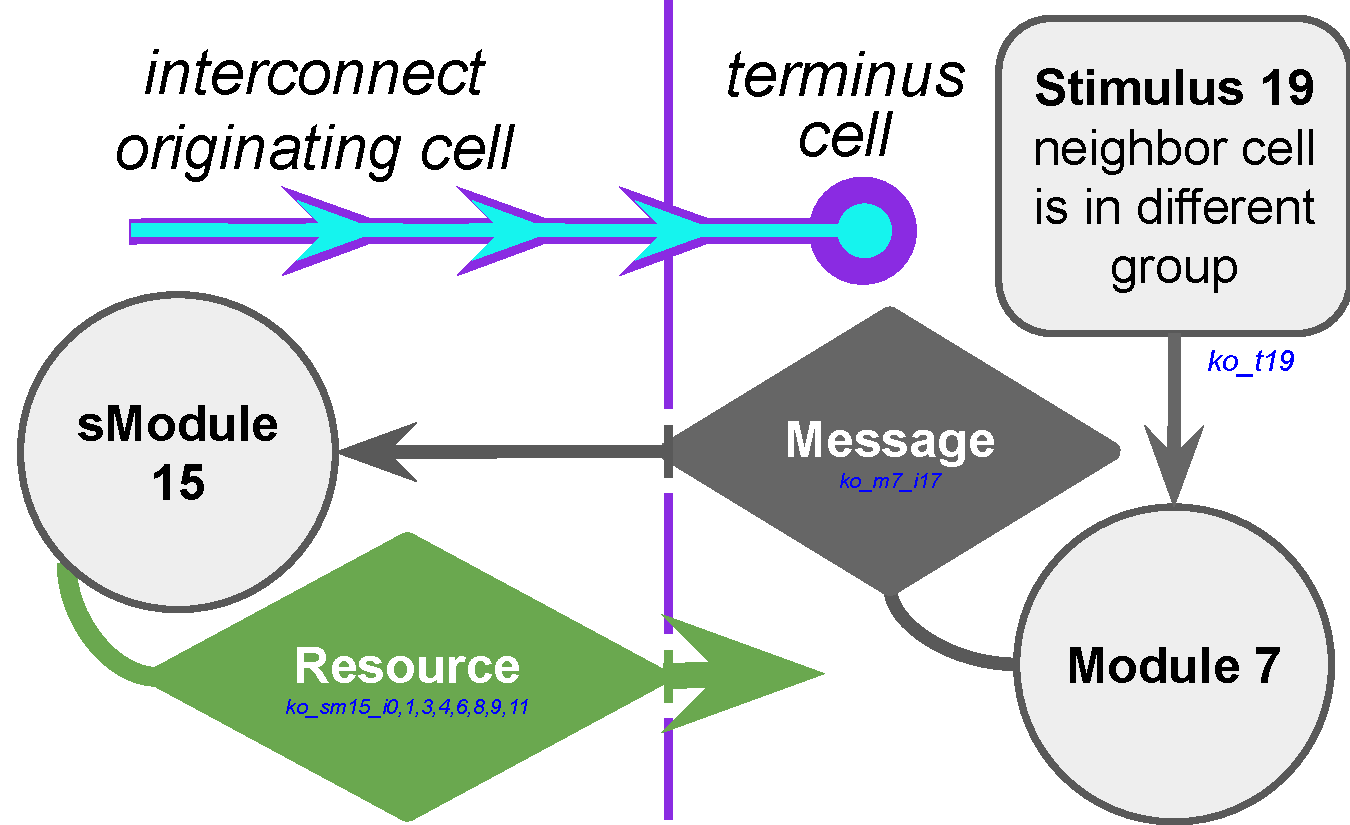
\includegraphics[width=\linewidth,clip]{batch=1042+step=1024+pop=3/1042_diagram}
  \caption{Hypothesized resource-recruiting mechanism}
  \label{fig:mechanism1}
\end{subfigure}
\begin{subfigure}[b]{0.45\linewidth}
  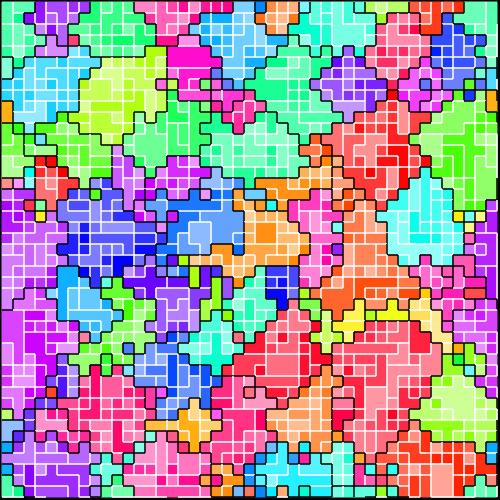
\includegraphics[width=\linewidth,trim={0 200 200 0},clip]{batch=1042+step=1024+pop=3/seed=1+title=channel+treat=batch_1042,step_1024,pop_3,id1_wt+update=4990+_emp_hash=0c549f0-clean+_source_hash=a6072a6-clean+ext=}
  \caption{Kin groups}
  \label{fig:kingroups1}
\end{subfigure}
\begin{subfigure}[b]{0.45\linewidth}
  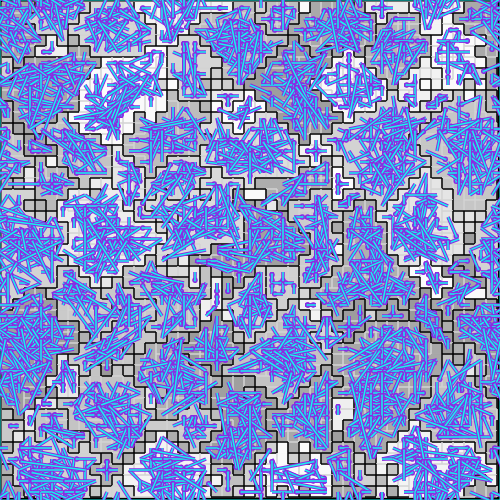
\includegraphics[width=\linewidth,trim={0 200 200 0},clip]{batch=1042+step=1024+pop=3/seed=1+title=established-interconnect+treat=batch_1042,step_1024,pop_3,id1_wt+update=4990+_emp_hash=0c549f0-clean+_source_hash=a6072a6-clean+ext=}
  \caption{Established interconnects}
  \label{fig:establishedinterconnects1}
\end{subfigure}
\begin{subfigure}[b]{0.45\linewidth}
  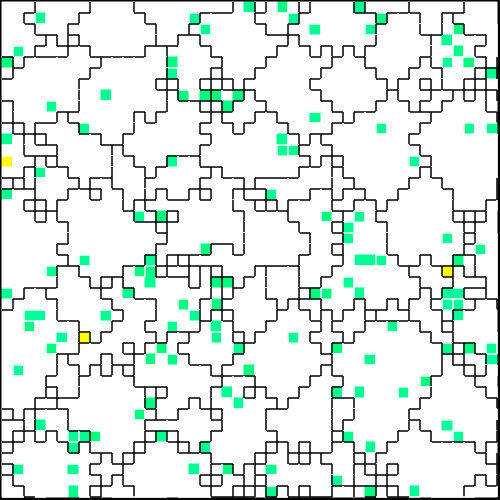
\includegraphics[width=\linewidth,trim={0 200 200 0},clip]{batch=1042+step=1024+pop=3/seed=1+title=interconnect-sharing-fraction+treat=batch_1042,step_1024,pop_3,id1_wt+update=4990+_emp_hash=0c549f0-clean+_source_hash=a6072a6-clean+ext=}
  \caption{Distribution of resource-sending cells}
  \label{fig:resourcesendingdistribution}
\end{subfigure}
\begin{subfigure}[b]{0.45\linewidth}
  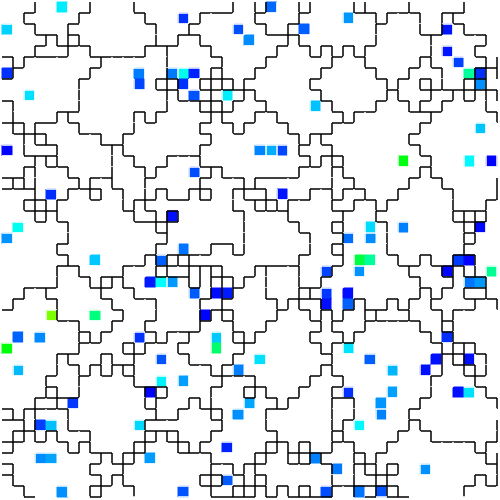
\includegraphics[width=\linewidth,trim={0 200 200 0},clip]{batch=1042+step=1024+pop=3/seed=1+title=interconnect-shared-resource+treat=batch_1042,step_1024,pop_3,id1_wt+update=4990+_emp_hash=0c549f0-clean+_source_hash=a6072a6-clean+ext=}
  \caption{Distribution of resource-receiving cells}
  \label{fig:resourcereceivingdistribution}
\end{subfigure}
\caption{
Batch 42 case study overview.
Figures \ref{fig:kingroups1} through \ref{fig:resourcereceivingdistribution} are generated from a snapshot of a wild-type strain monoculture population.
In these images, each grid tile represents an individual cell.
Cells are organized into kin groups, color-coded by hue in Figure \ref{fig:kingroups1}.
Established interconnects are overlaid in blue on Figure \ref{fig:establishedinterconnects1}.
In Figures \ref{fig:resourcesendingdistribution} and \ref{fig:resourcereceivingdistribution}, kin groups are outlined in black.
Figure \ref{fig:resourcesendingdistribution} highlights cells that are sending resource over-interconnect.
Figure \ref{fig:resourcereceivingdistribution} highlights cells that are receiving resource over-interconnect.
You can view an animation of the wild-type monoculutre at \url{https://mmore500.com/hopto/ao}.
}
\label{fig:case_study_1042}
\end{center}
\end{figure}
